\clearpage
\thispagestyle{empty}
~\clearpage
%\graphicspath{{Figures_chapter-4/}}
%\chapter{New Finite Difference Approach Involving Interfacial Points For Solving Immersed Interface Problems And Its Application to Stokes Flows}
%\chapter{New Finite Difference Approach Involving Interfacial Points For Solving Arbitrary Shaped Interface Problems in Cartesian Coordinates}
%\chapter{Interfacial Points Based Finite Difference Scheme For Solving Interface Problems in Cartesian Coordinates}
\chapter{Case Study II}
\label{chap5}
\section{Experiment Design}
In our study, we demonstrated the ability of HackIT tool as a single-player platform for conducting experiments. The network topology was manipulated across three rounds: RDS configuration (N = 6), Non-RDS configuration (N = 6) and mixed configuration (N=6). The total number of servers were 40, where 30 web-servers were assigned as honeypot web-servers. Across three configuration, participants playing as hackers were given 20 minutes to probe and exploit.

In this experiment, 


if the timing of deception was early, then deception was present on the second and third rounds in the sequence. However, if the timing of deception was late, then deception was present in the fourth and fifth rounds in the sequence as shown in Figure \ref{fig:figure8}. The honeypots were easy to exploit via common ports and vulnerabilities in the deception rounds compared to the non-deception rounds, where there were no honeypots. However, participants were not told that honeypots will involve easy to attack configurations in deception rounds. Also, participants were not disclosed the rounds on which deception was involved. To analyze human data, we looked at the proportion of honeypot attacks and proportion of regular attacks at the attack stage by the hacker across six-rounds in each condition. These proportions were calculated by average the attack decision over all the trials and participants. We also calculated frequency of each exploits used on regular and honeypots in deception and no-deception trials.

\section{HackIT Task}
The objective of attacker in HackIT was to steal real credit-card information located on webservers.We configured the network with 40 webservers where 30 webservers acted as honeypots.The participants were given 20 minutes to probe and exploit the network.We used different configurations shown in \ref{fig:figure7}. For example, a system with Windows XP operating system, port 80/tcp, and service http was easily exploitable. Such a configuration was mapped to a honeypot. However, a system with Linux operating system, port 22/tcp and service ssh was difficult to
attack. Such a configuration was mapped to a regular webserver. Participants were informed about the easy to exploit and the difficult to exploit configurations in the output of the \textit{nmap} command. The participants could \textit{exit} the game anytime. Attacking the real webserver granted 100 game points while attacking the honeypot resulted in the loss of 100 game points. The score of a participant was only displayed when either the time expired or the participant left the game.

\FloatBarrier
\begin{figure}[!htbp]
\centering
  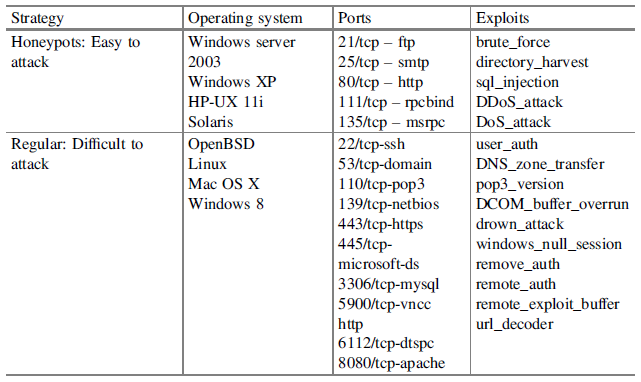
\includegraphics[scale=0.6]{Chap3/exploits.PNG}
  \caption{Configuration of honeypot and regular system}\label{fig:figure7}
\end{figure} 
First, the attacker probed the network using nmap command to gain information about different web-servers. Probing different web-servers gave the information about the operating system, open ports, services, and vulnerabilities. The information provided to the attacker as a result of probing systems gave him an idea about the type of configuration on the probed system. Once the attacker collects information about open ports and services, he could attack a web-server by using the \enquote{use\_exploit} command.
The use\_exploit command exploited vulnerabilities on a system and helped the attacker to gain access to that web-server. Next, the attacker could list different files on the exploited web-server by using the “ls” command. Next, the attacker could transfer required files containing credit card information (e.g., \enquote{pin.txt}) using the \enquote{scp} command. After attackers copied the file from the exploited system, he was informed whether he was successful or not in stealing a real credit-card file from the computer via a text-based feedback.
\section{Participants}
Participation was voluntary and a total of 18 male participants participated in the study that was advertised via an email advertisement. Out of the 18 people, 78\% people had taken a course in computer networks/security. The age of participants ranged from 18\textendash 22 years. About 6\% were 3rd year and 94\% were final year undergraduate students from Indian Institute of Technology Mandi, India. All the participants were remunerated at a fixed rate of INR 20 for their participation in the study along with Amazon gift coupons for top scorers.

\section{Procedure}
Participants were given instructions about their objective in the HackIT task, and they were informed about their own action’s payoffs. Specifically, human hackers were asked to maximize their payoff by stealing the real credit-card file from the network over the course of 20 minutes. During the Probe stage Hacker could probe the network using \enquote{nmap} utility . After probing the web-servers, he received information about open ports, operating systems, services, and vulnerabilities associated with different web-server. Next, the hacker had to choose one web-server to exploit and exploit web-servers using “use\_exploit” command during attack stage. Once the web-server was exploited, hackers transferred the credit-card file to their remote computer.The goal was to maximize the score in the duration of 20 minutes. The participants could \textit{exit} the game anytime.The participants were divided into group of 6 with total number of groups being 3 based on the three different network configurations. Different groups were given different network topologies and different virtual views of the hosts. Finally, we compared the results across the 3 different configurations.

\section{Results and Analysis}
Figure \ref{fig:figure21} shows the host detection rate of real hosts across the 3 different network configurations RDS, Mixed and Non-RDS. Host detection rate signifies the proportion of real nodes that are exploited out of all the real nodes within the network. Hence, a host detection rate of 0.2 will mean that 2 of the real nodes have been exploited, since our network contains a total of 10 real nodes across all the configurations.

\FloatBarrier
\begin{figure}[!htbp]
\centering
  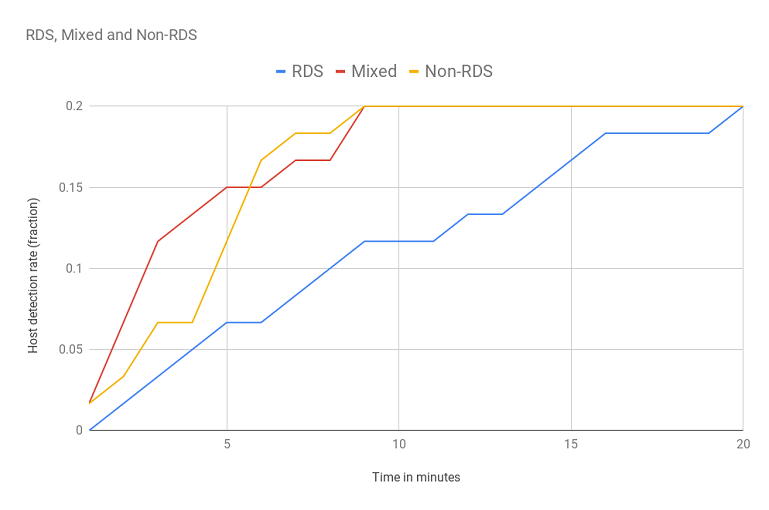
\includegraphics[scale=0.7]{Chap5/single.png}
  \caption{Host detection rate(Real) v/s the Time taken}\label{fig:figure21}
\end{figure}

From Figure \ref{fig:figure21}, we can infer that RDS is better at delaying the detection of hosts. For any point in time, we can see that our RDS has a lower host detection rate compared to the other two configurations. This proves that RDS is a more effective configuration than Non-RDS as well as the mixed configuration.

\FloatBarrier
\begin{figure}[!htbp]
\centering
  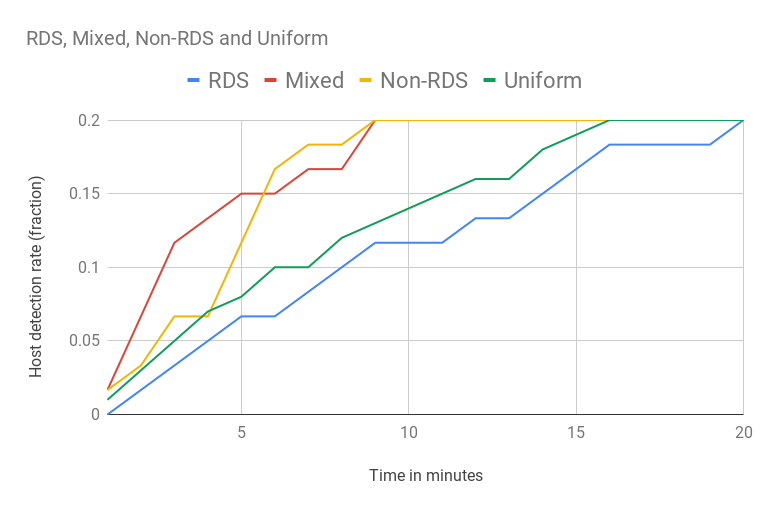
\includegraphics[scale=0.55]{Chap5/uniform.png}  \caption{Uniform Scanning}\label{fig:figure22}
\end{figure}
\FloatBarrier
\begin{figure}[!htbp]
\centering
  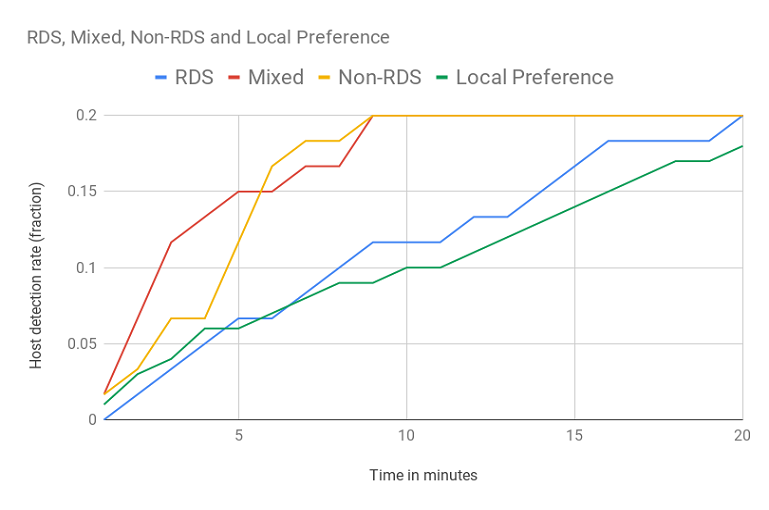
\includegraphics[scale=0.65]{Chap5/local.png}  \caption{Local Preference Scanning}\label{fig:figure23}
\end{figure}
\FloatBarrier
\begin{figure}[!htbp]
\centering
  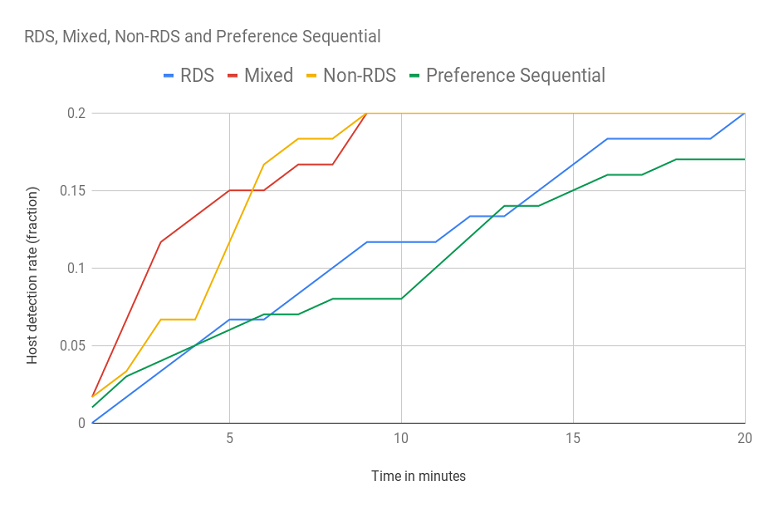
\includegraphics[scale=0.7]{Chap5/prefseq.png}  \caption{Preference Sequential Scanning}\label{fig:figure24}
\end{figure}
\FloatBarrier
\begin{figure}[!htbp]
\centering
  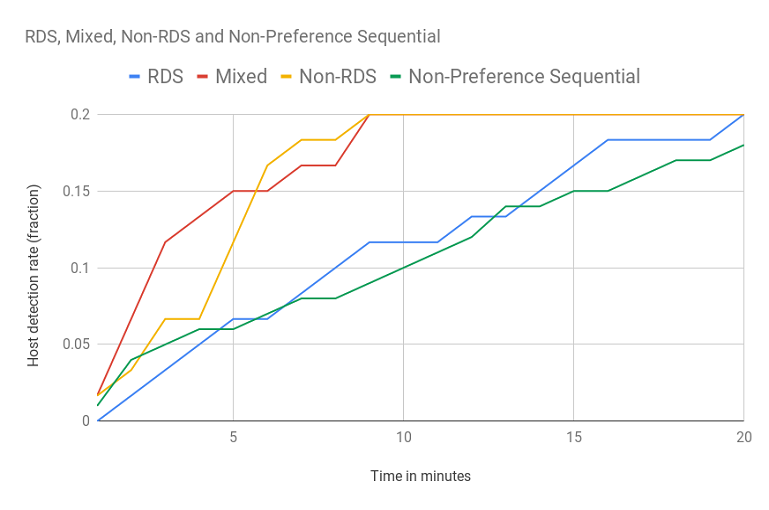
\includegraphics[scale=0.7]{Chap5/nonpref.png}  \caption{Non-Preference Sequential Scanning}\label{fig:figure25}
\end{figure}
\FloatBarrier
\begin{figure}[!htbp]
\centering
  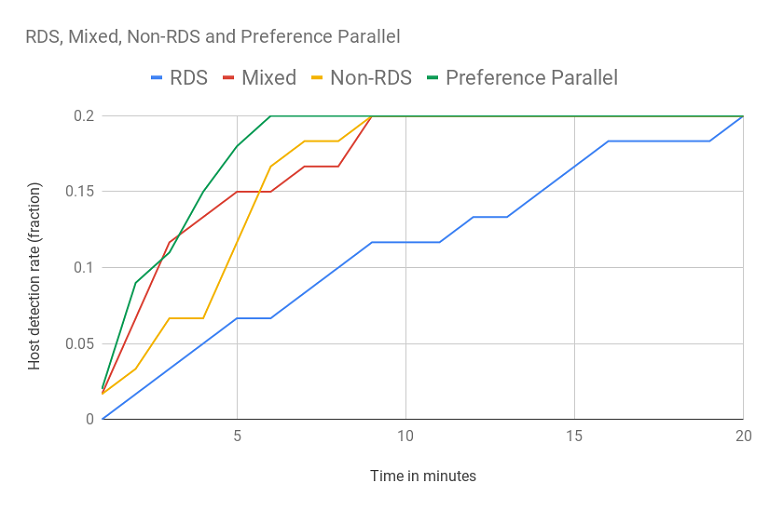
\includegraphics[scale=0.7]{Chap5/prefpar.png}  \caption{Preference Parallel Scanning}\label{fig:figure26}
\end{figure}

\bgroup
\def\arraystretch{1.5}
\begin{table}[]
\centering
\begin{tabular}{|c|c|c|c|}
\hline
\textbf{Type of Scanning} & \textbf{RDS} & \textbf{Mixed} & \textbf{Non-RDS} \\
\hline
\textbf{Local Preference} & 0.0174642492  & 0.07139094247 & 0.06861324783 \\ \hline
\textbf{Uniform} & 0.02089657069 & 0.04391279237 & 0.03986783722 \\ \hline
\textbf{Non-Preference Sequential} & 0.01663329993 & 0.06808083431 & 0.06592504161 \\ \hline
\textbf{Preference Sequential} & 0.01852925615 & 0.07292690404 & 0.06997221671 \\ \hline
\textbf{Preference Parallel} & 0.07534365711 & 0.02045319861 & 0.03129607714 \\ \hline
\end{tabular}
\caption{ Root Mean Square Error for all the scanning techniques with user data}
\label{tab:my-table}
\end{table}
\egroup

\clearpage